\chapter{Experiments and Evaluation}
In this chapter, we describe our experiments regarding to 2 research questions we proposed on chapter 1. The experiment based on the DevOps toolchain we implemented in the Chapter 4. In the experiments we compared the implementation on serverless with the implementation on traditional VM based cloud infrastructure. Thus in experiments, we also implement the solution with different type of cloud environment (with/without serverless) as a comparison group.
\par
In the first experiment we will examine how does the serverless compute engine for containers (Amazon ECS on AWS Fargate) could be used in continuous delivery pipeline(in our case, Jenkins) -- the core element of our DevOps toolchain. The second experiment shows how does serverless functions (AWS lambada) could be used in DevOps toolchain. The last experiment focus on answering research question 2, in which we will using compared continuous delivery pipeline composed with fully-managed serverless DevOps tools in AWS with our Jenkins-based pipeline that runs on the virtual machine.
\section{Experiment on Managed Container Services}
This experiment is a controlled experiment which examine how serverless container service could affect the continuous delivery pipeline from various perspectives.
\subsection{Test task and System Description}
In this experiment we run the continuous delivery process of a Spring Boot web application with our DevOps toolchain. From the experiments, we could verify our assumption in CH3, and better answering research question 1.
\par
As we described in Chapter 4, the continuous delivery pipeline includes following steps:
\begin{enumerate}
    \item \textit{Checkout}: Pull the most recent change from Github repository
    \item \textit{Build}: Build the application with Gradle, with automate testing with JUnit integrated in Gradle.
    \item \textit{Build the docker image}: Build the docker image of our Spring Boot application.
    \item \textit{Push to Container Registry}: Push the docker image from last step to the AWS elastic cloud registry (ECR) for the further deployment.
\end{enumerate}
\par
In these 4 steps, the step "Build" and "Checkout" is being done in parallel with in the ECS cluster. As we mentioned in CH4, when new job started in the Jenkins master server, jenkins will provisioning new container instance within the ECS cluster. The container is managed directly by AWS, so we don't need to create and manage the virtual machine that runs the container. We use this setup in our initial implementation as the control group.
\par
In experimental group we replace AWS Fargate with traditional VM, which is EC2 in the Amazon Web Services. We manually create EC2 virtual machines and let Jenkins runs the same continuous delivery pipeline on it. The parallelization pattern remain the same, this means as in the controlled group, only first two steps are being run distributively in the Jenkins nodes.
\par
Figure \ref{fig:ex1} shows the architecture with in 2 groups in this experiment. The experimental group on the left is a Jenkins server with traditional virtual machine as worker agents. The architecture of controlled group on the right has agent nodes dynamically provisioned as serverless containers hosed by AWS Fargate.
\subsubsection{Hardware}
The hardware of Jenkins agents is the independent variable that exposed to the change in the experiment.
\par
The experiments are conducted on Amazon Web Services (AWS). The hardware of Jenkins master node in both experiment groups is the same, which is EC2 instance of type t3.small with 2 virtual cpu, 2 GB RAM and 30 GB disk. Each EC2 instance has 2 Jenkins executer according to the Jenkins default setting. This means 2 container could run in parallel on each EC2 virtual machine.
\par
In the control group, which is the implementation we presented in CH4, the Jenkins agents runs on AWS ECS powered by AWS Fargate. The virtual hardware resources that are allocated to each serverless container is 1 virtual cpu, and 1 GB of RAM. This make sure that each container shares the same hardware resources as in another group, so the hardware will not affect the result.
\subsubsection{Software}
We maintain the same software setup in each group. The operation System for EC2 instance that runs Jenkins master node is Ubuntu Server 18.04. The version of Jenkins that runs on the server is 2.222.3. For connect ECS and Fargate which works as the Jenkins agents, we use Jenkins plugin Amazon Elastic Container Service (ECS) / Fargate, version 1.34. The container in Fargate/EC2 for running the Checkout and Build steps is from our own developed docker image which you can find at \footnote{https://hub.docker.com/r/dry1995/jnlp}. The docker image includes essential dependencies that will be used for build the Spring Boot application, and the base image which allow container connects Jenkins master as an agent. 
\begin{figure}[h]
    \centering
    \begin{minipage}{0.45\textwidth}
        \centering
        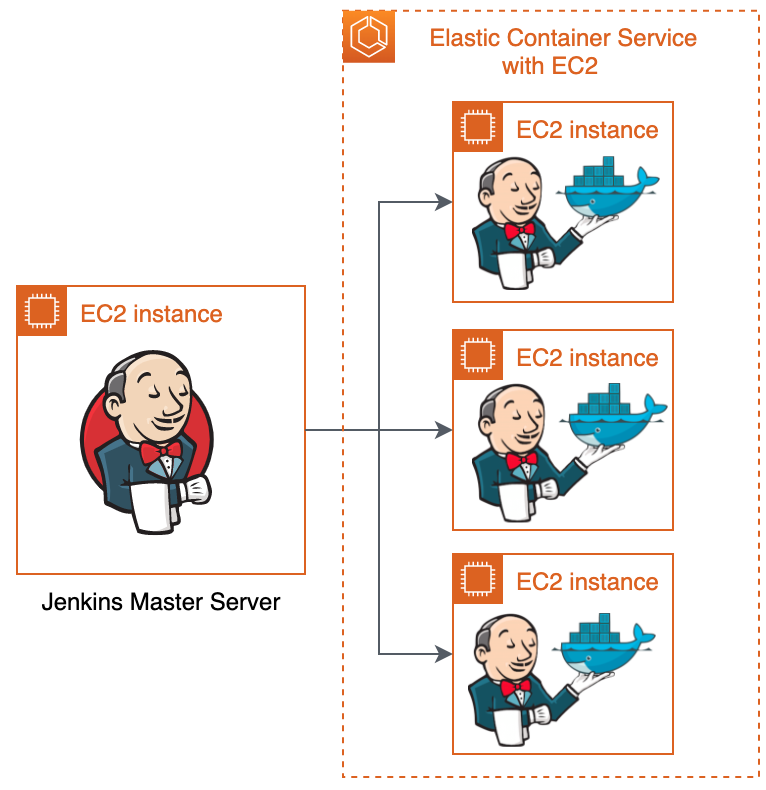
\includegraphics[width=\textwidth]{pics/jenkins-on-vm.png} % first figure itself
    \end{minipage}\hfill
    \begin{minipage}{0.54\textwidth}
        \centering
        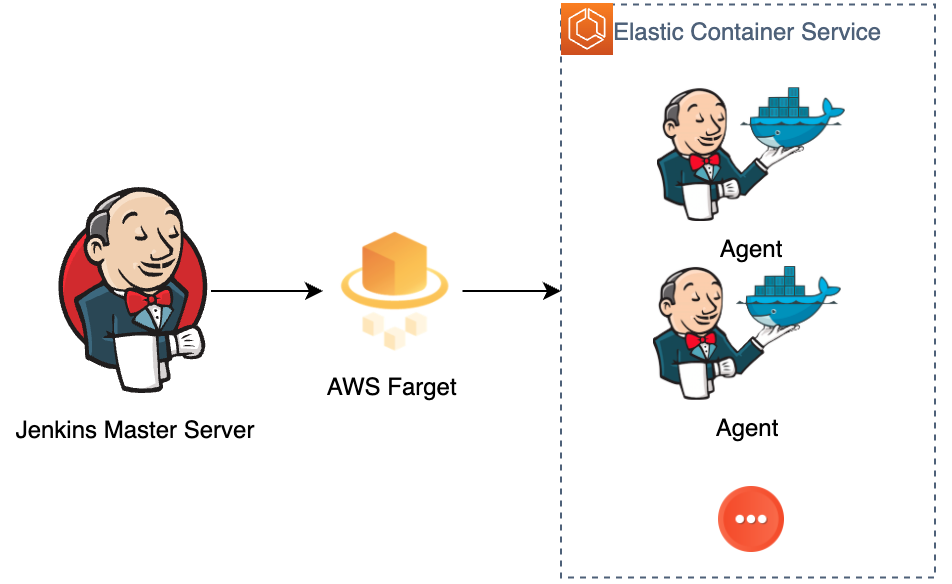
\includegraphics[width=\textwidth]{pics/jenkins-on-fargate.png} % second figure itself
    \end{minipage}
    \label{fig:ex1}
    \caption{Architecture diagram of the test Jenkins cluster with agents running in traditional virtual machine (left) and on ECS with AWS Fargate (right)}
\end{figure}
\subsection{Performance Properties and Evaluation}
We run the pipeline through 2 different setups, we will get the result of following properties:
\begin{itemize}
    \item \textit{Runtime} describes the total time for finishing all the tasks.
    \item \textit{Cost Structure} describes the daily cost of 2 setups under the same workload
    \item \textit{Resource Utilization} describes the average CPU/RAM usage for each instance during a single run of the pipeline.
\end{itemize}
To shows how does the 2 setups performance within the teams with different sizes, we run by run different number of tasks parallel through the pipeline. This simulates the different team size, besides, it could also shows the scalability when comes to the need of task parallelization in bigger organizations.
